

	
\documentclass{article}
\usepackage{longtable}
\usepackage[acronym]{glossaries}
\usepackage{graphicx}


	

% abbreviations:
\newacronym{ropod}{ropod}{Robotic Pod}
\newacronym{smartwheel}{SW}{Smart wheel}


% nomenclature:
\newglossaryentry{Inertialframe}{
	name = $(*)^I$ ,
	description = Superscript describing that $(*)$ is expressed in the Inertial coordinate frame,
}

\newglossaryentry{Ropodframe}{
	name = $(*)^R$ ,
	description = Superscript describing that $(*)$ is expressed in the Robot coordinate frame,
}
\newglossaryentry{Wheelframe_i}{
	name = $(*)^W_i$ ,
	description =  Superscript and subscript describing that $(*)$ is expressed in the coordinate frame of Smart-Wheel $i$,
}
\newglossaryentry{W_wheels}{
	name = $W_i$ ,
	description =  Point at which Smart-Wheel $i$ is connected to the Robot frame,
}

\newglossaryentry{C_robot}{
	name = $C$ ,
	description =  Center of mass of the robot frame,
}

\newglossaryentry{O_robot}{
	name = $O$ ,
	description =  Center of the intertial coordinate frame,
}

\newglossaryentry{Dist_wheels}{
	name = $d_w$ ,
	description =  Distance between wheels in a smartwheel,
}
\newglossaryentry{Offs_wheels}{
	name = $s_w$ ,
	description =  Offset of the rotation point of the smartwheel relative to the axis connecting the wheels,
}

\newglossaryentry{r_wheels}{
	name = $r_w$ ,
	description =  Wheel radius,
}

\newglossaryentry{x}{
	name = $x$ ,
	description =  $x$-position of the robot center of mass C in the intertial coordinate frame,
}

\newglossaryentry{y}{
	name = $y$ ,
	description =  $y$-position of the robot center of mass C in the intertial coordinate frame,
}

\newglossaryentry{theta}{
	name = $\theta$ ,
	description =  Orientation angle of the robot in the intertial coordinate frame,
}

\newglossaryentry{delta_i}{
	name = $\delta_i$ ,
	description =  Orientation angle of the Smart-Wheel coordinate frame with respect to the robot coordinate frame,
}

\newglossaryentry{varphi_ilr}{
	name = $\varphi_{i,l/r}$ ,
	description =  Rotation angle of the left/right wheels in a Smart-Wheel from an observer situated at $W_i$ and looking towards axis $X_i^W$,
}

\newglossaryentry{v_ilr}{
	name = $v_{i,l/r}$ ,
	description =  Translation velocity of the left/right wheel in a Smart-Wheel from an observer situated at $W_i$ and looking towards axis $X_i^W$,
}

\newglossaryentry{q}{
	name = $q$ ,
	description =  position vector of the robot in generalized coordinates\, i.e. in the intertial coordinate frame,
}

\newglossaryentry{v}{
	name = $v$ ,
	description =  vector comtaining all wheels velocities of a ropod,
}

\makeglossaries
\begin{document}
    \glsaddall
	
	
	\printglossary[type=\acronymtype,title=Abbreviations,nonumberlist]
	
	\printglossary[title=Nomenclature,nonumberlist]
	\newpage
	
	
	The \gls{smartwheel} and its respective coordinate frame are shown in Fig. \ref{fig:Smartwheel}.
\begin{figure}[h]
	\centering
	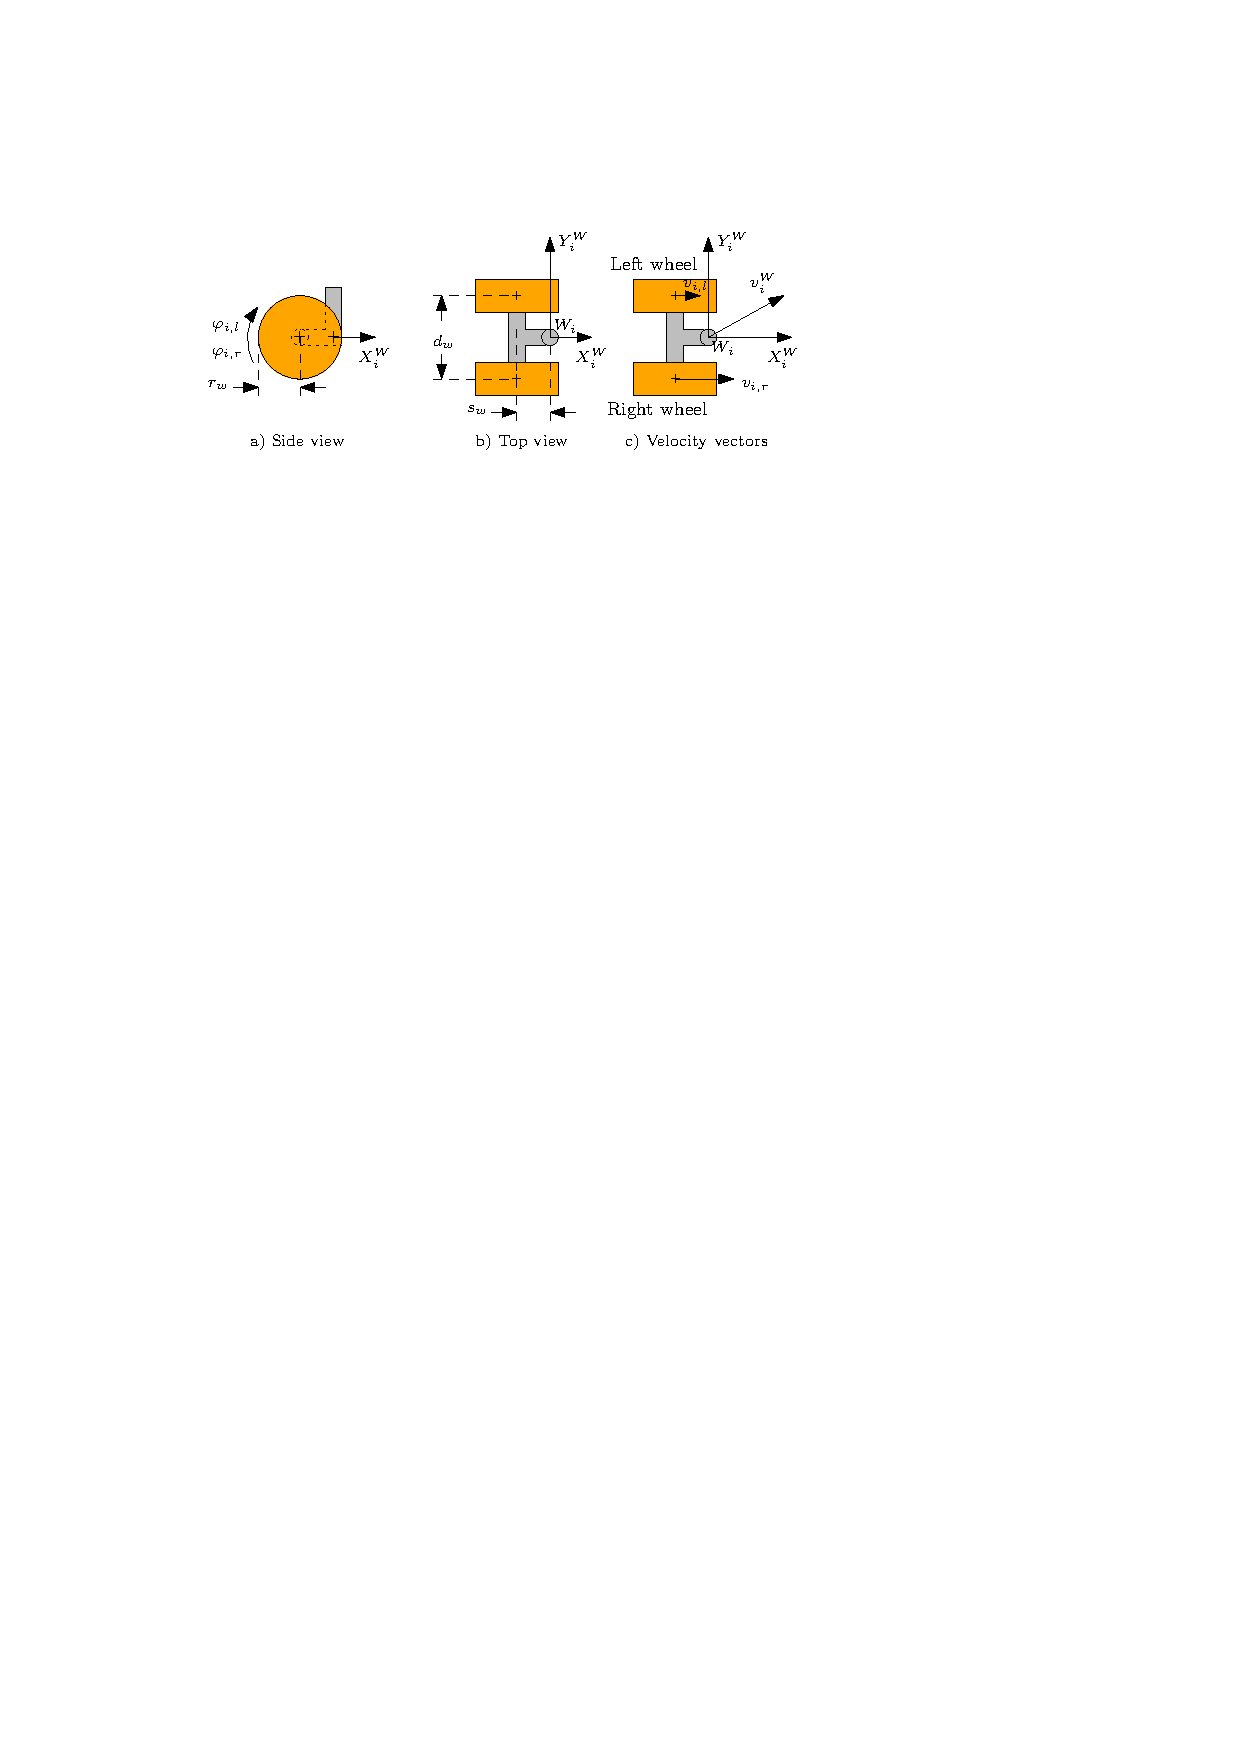
\includegraphics[]{Smartwheel.pdf}
	\caption{Smartwheel}
	\label{fig:Smartwheel}
\end{figure}

The wheels of the \gls{smartwheel} have rotation angles \gls{varphi_ilr} for the left and right wheel respectively. The corresponding wheel translation velocities are denoted by \gls{v_ilr}, these are scalars since at this point no wheel sleep is considered.\\

A \gls{ropod} consists of several \gls{smartwheel}s attached with a rigid frame with center of mass located at \gls{C_robot}. The initial design of a \gls{ropod} have four \gls{smartwheel}s and are ordered as depicted in Fig.\ref{fig:Smartwheel_ord}. 

	\begin{figure}[h]
		\centering
		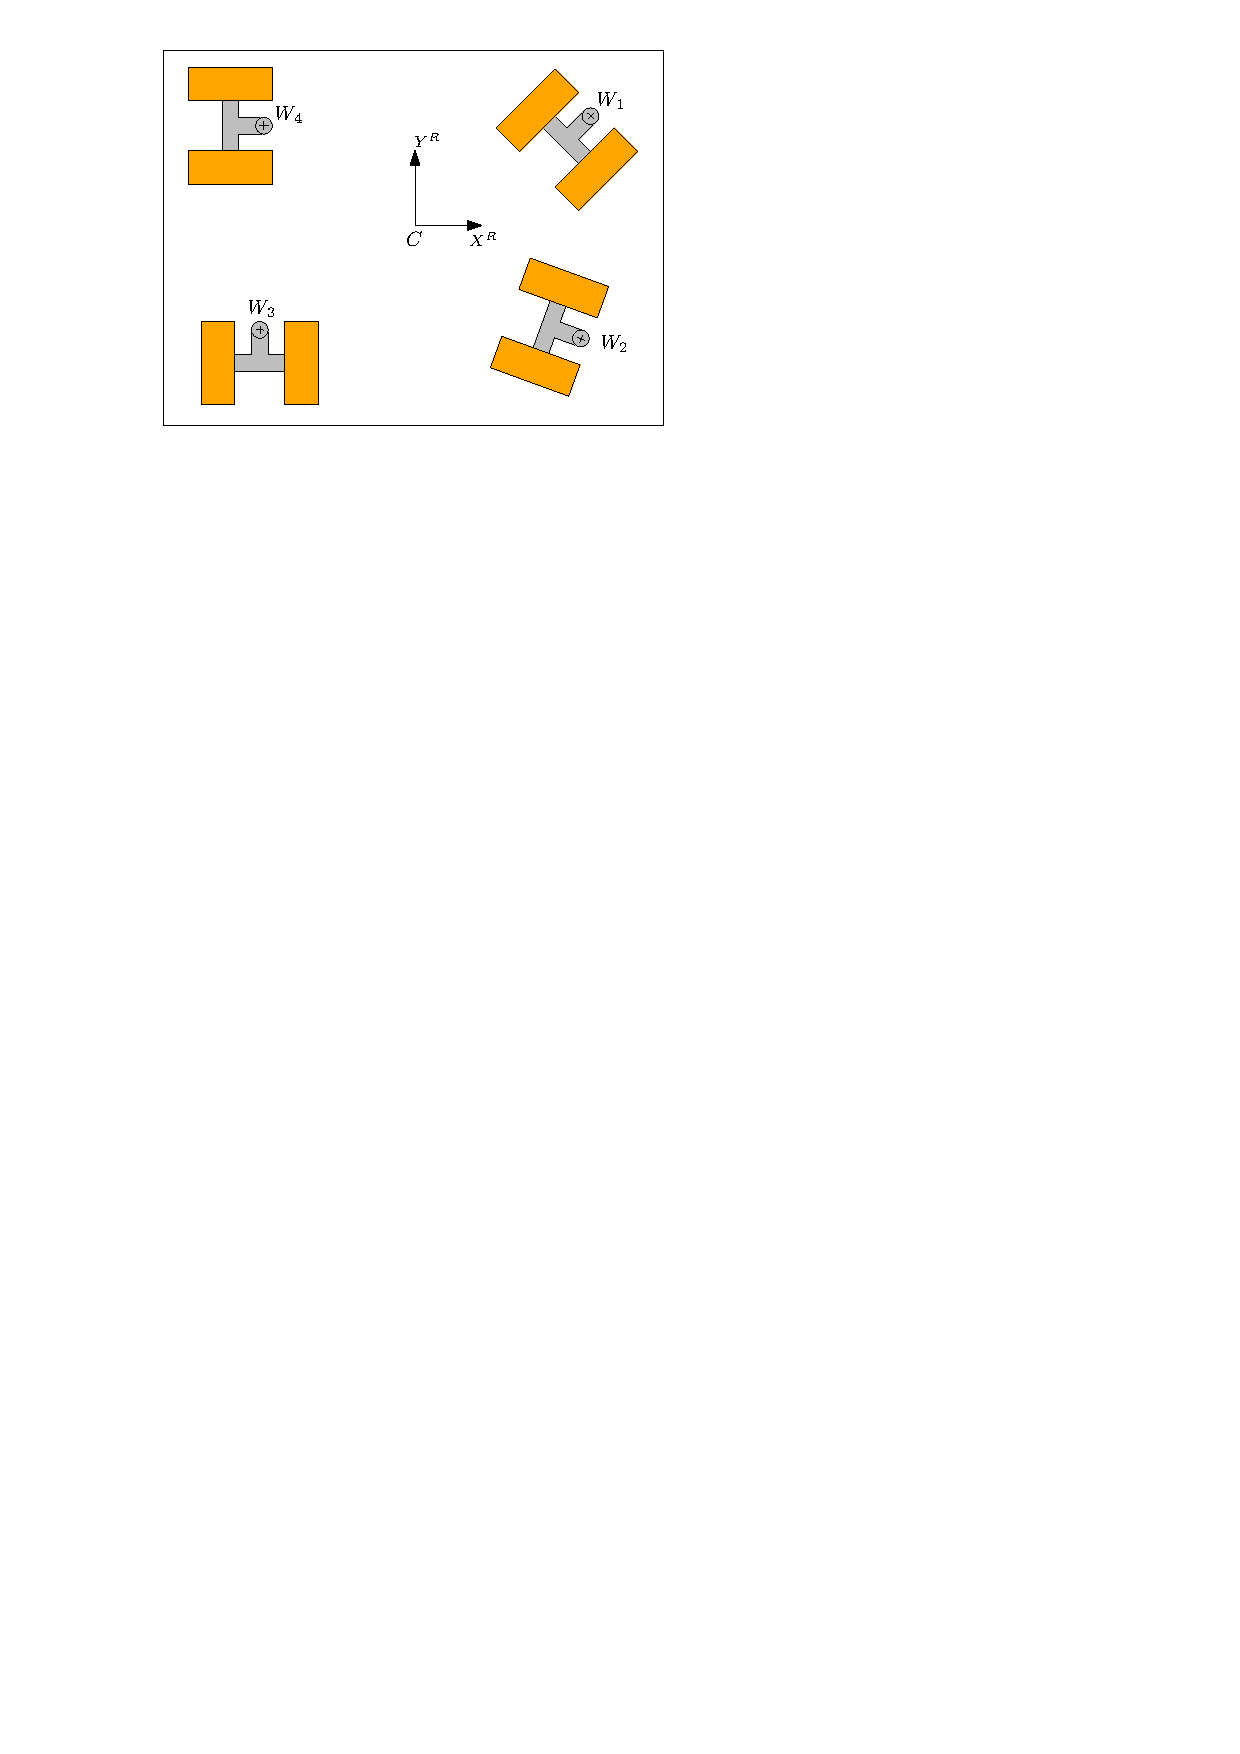
\includegraphics[]{Ropod_wheelorder.pdf}
		\caption{Smart-wheel order convention}
		\label{fig:Smartwheel_ord}
	\end{figure}

The relation between the \gls{smartwheel}, robot and inertial coordinate frames is shown in Fig.\ref{fig:Ropod_coordinates}. 

	\begin{figure}[h]
		\centering
		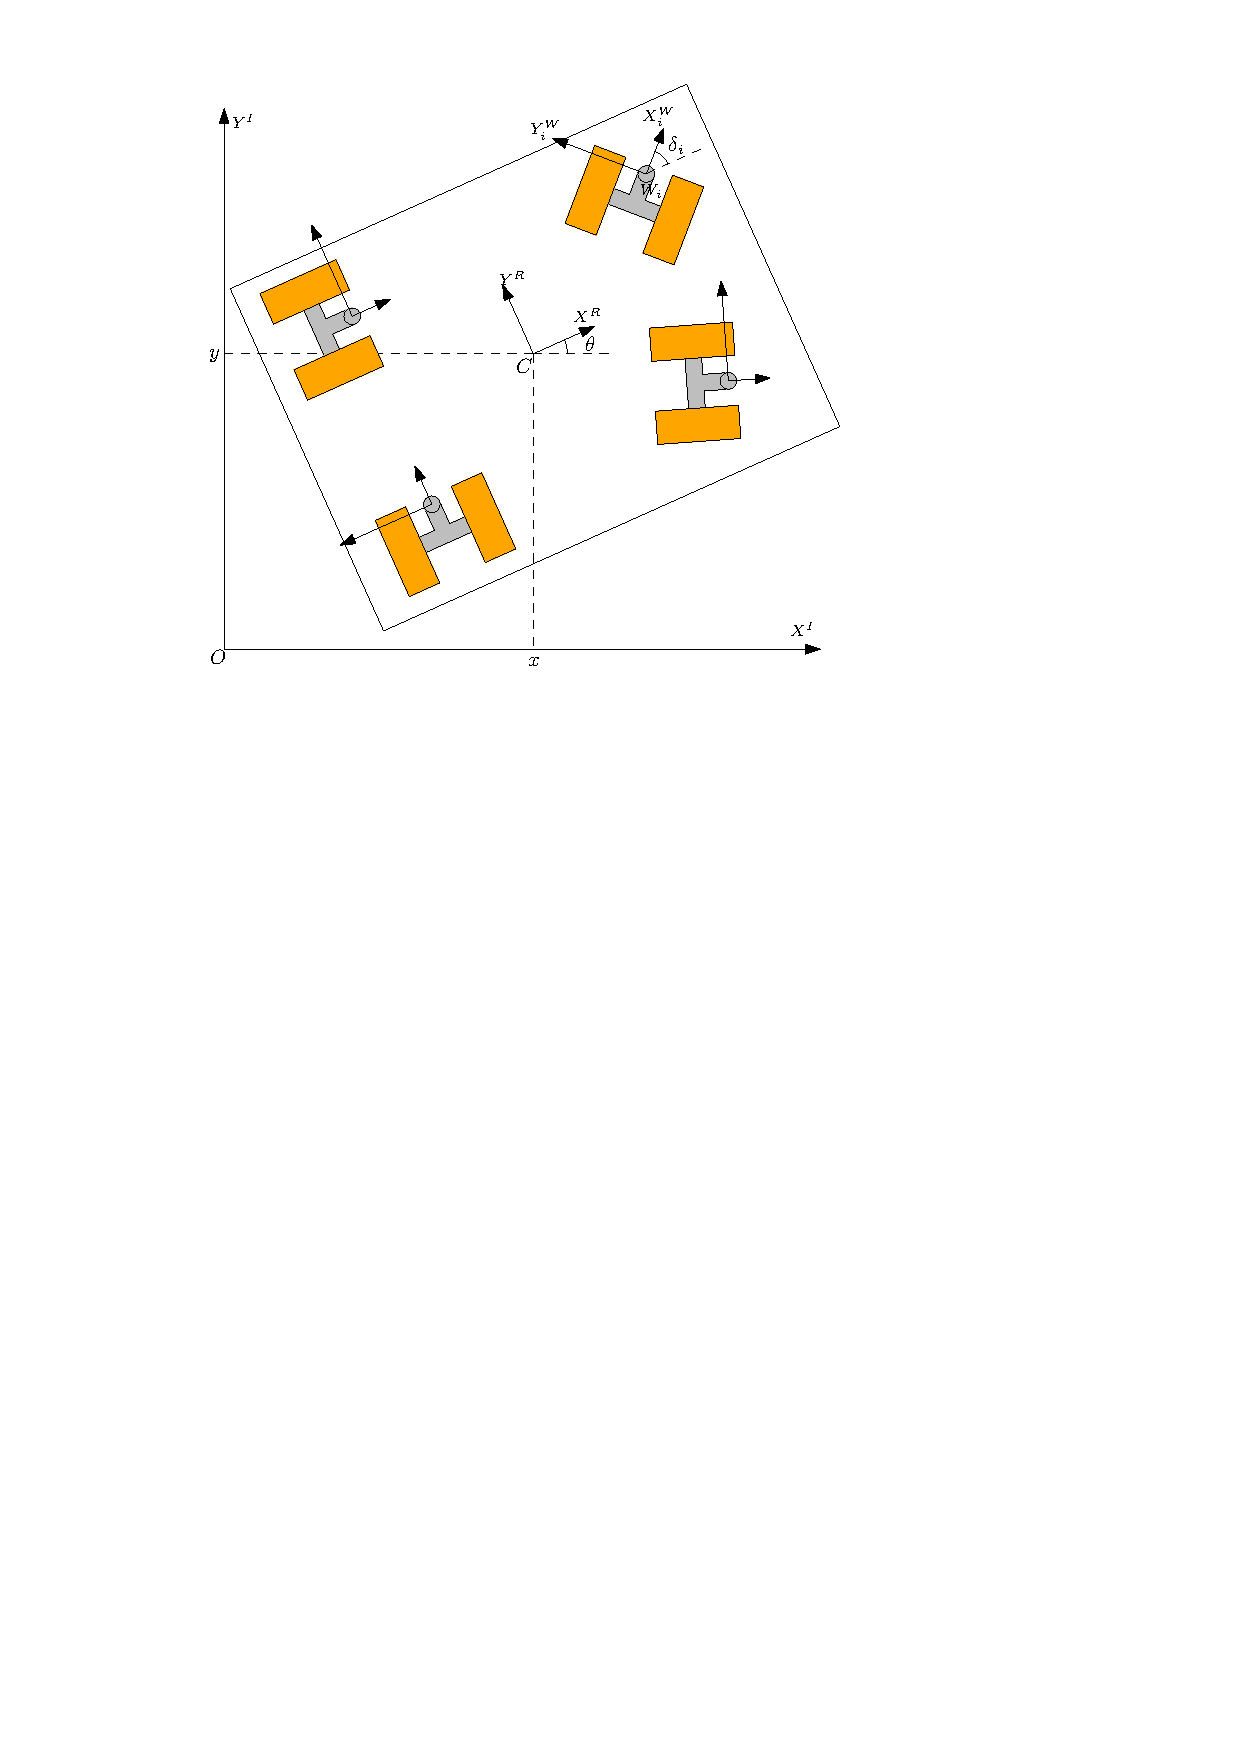
\includegraphics[]{Ropod.pdf}
		\caption{RoPod coordinate frames convention.}
		\label{fig:Ropod_coordinates}
	\end{figure}
	


    

\end{document}	

	\printacronyms[include-classes=abbrev,name=Abbreviations]
	
	\printacronyms[include-classes=nomencl,name=Nomenclature]
	
	
\end{document}